% Nejprve uvedeme tridu dokumentu s volbami
\documentclass[slovak,bachelorpractice,dept460,male,csharp,cpdeclaration]{diploma}
% Dalsi doplnujici baliky maker
\usepackage[autostyle=true,czech=quotes]{csquotes} % korektni sazba uvozovek, podpora pro balik biblatex
\usepackage[backend=biber, style=iso-numeric, alldates=iso]{biblatex} % bibliografie
\usepackage{dcolumn} % sloupce tabulky s ciselnymi hodnotami
\usepackage{subfig} % makra pro "podobrazky" a "podtabulky"

% Zadame pozadovane vstupy pro generovani titulnich stran.
\ThesisAuthor{Miroslav Kačeriak}
\SubmissionDate{\today}

\Thanks{\textcolor{red}{Rád bych na tomto místě poděkoval všem, kteří mi s prací pomohli, pretože bez nich by tato práce nevznikla.}}


% Zadame cestu a jmeno souboru ci nekolika souboru s digitalizovanou podobou zadani prace.
% Pokud toto makro zapoznamkujeme sazi se stranka s upozornenim.
%\ThesisAssignmentImagePath{Figures/Assignment}

% Zadame soubor s digitalizovanou podobou prohlaseni autora zaverecne prace.
% Pokud toto makro zapoznamkujeme sazi se cisty text prohlaseni.
%\AuthorDeclarationImageFile{Figures/AuthorDeclaration.jpg}


% Zadame soubor s digitalizovanou podobou souhlasu spolupracujici prav. nebo fyz. osoby.
% Pokud toto makro zapoznamkujeme sazi se cisty text souhlasu.
%\CooperatingPersonsDeclarationImageFile{Figures/CoopPersonDeclaration.jpg}


\CzechAbstract{\textcolor{red}{Tohle je český abstrakt, zbytek odstavce je tvořen výplňovým textem. Naší si rozmachu potřebami s posílat v poskytnout ty má plot. Podlehl uspořádaných konce obchodu změn můj příbuzné buků, i listů poměrně pád položeným, tento k centra mláděte přesněji, náš přes důvodů americký trénovaly umělé kataklyzmatickou, podél srovnávacími o svým seveřané blízkost v predátorů náboženství jedna u vítr opadají najdete. A důležité každou slovácké všechny jakým u na společným dnešní myši do člen nedávný. Zjistí hází vymíráním výborná.}}

\CzechKeywords{typografie; \LaTeX; diplomová práce}

\EnglishAbstract{\textcolor{red}{This is English abstract. Lorem ipsum dolor sit amet, consectetuer adipiscing elit. Fusce tellus odio, dapibus id fermentum quis, suscipit id erat. Aenean placerat. Vivamus ac leo pretium faucibus. Duis risus. Fusce consectetuer risus a nunc. Duis ante orci, molestie vitae vehicula venenatis, tincidunt ac pede. Aliquam erat volutpat. Donec vitae arcu. Nullam lectus justo, vulputate eget mollis sed, tempor sed magna. Curabitur ligula sapien, pulvinar a vestibulum quis, facilisis vel sapien. Vestibulum fermentum tortor id mi. Etiam bibendum elit eget erat. Pellentesque pretium lectus id turpis. Nulla quis diam.}}

\EnglishKeywords{typography; \LaTeX; master thesis}

\AddAcronym{PC}{Personal Computer}
\AddAcronym{OS}{Operating System}
\AddAcronym{RPG}{Role Playing Game}
\AddAcronym{EOS}{Epic Online Services}
\AddAcronym{CLR}{Common Language Runtime}
\AddAcronym{JIT}{Just-In-Time}
\AddAcronym{IL}{Intermediate Language}
\AddAcronym{XML}{eXtensible Markup Language}
\AddAcronym{WPF}{Windows Presentation Foundation}
\AddAcronym{LFS}{Large File Storage}

\addbibresource{literature.bib}

% Novy druh tabulkoveho sloupce, ve kterem jsou cisla zarovnana podle desetinne carky
\newcolumntype{d}[1]{D{,}{,}{#1}}

\begin{document}
\MakeTitlePages

% A nasleduje text zaverecne prace.
\section{Úvod}
\label{sec:Introduction}
V rámci mojej odbornej praxe som dostal možnosť nahliadnuť za oponu herného vývoja v českom nezávislom štúdiu Perun Creative. Nakoľko sa o hry a herný priemysel dlhodobo zaujímam, táto firma a jej tvorba mi bola vopred známa. Aj po prednáške jej dvoch spoluzakladateľov a zároveň programátorov, ktorá sa uskutočnila v priestoroch Vysokej školy báňskej, som bol stále prekvapený vysokou technologickou úrovňou ich prvého projektu. Firmu som chcel kontaktovať so žiadosťou o prácu nezávisle od odbornej praxe, no keď som sa dozvedel, že už niekoho práve na odbornú prax hľadajú, rozhodol som sa to využiť. Pracovnému pohovoru predchádzalo zaslanie programátorského portfólia zloženého zo školských ale aj vlastných prác. Samotný pohovor potom prebiehal online s oboma programátormi Bc. Jánom Polachom a Bc. Jirkou Vašicou, ktorí sa neskôr stali aj mojimi kolegami.

Do firmy som nastúpil na konci životného cyklu projektu, takže som sa nemohol podieľať na vývoji základných herných mechaník. Naopak to znamenalo nutnosť dôkladne sa s celým projektom zoznámiť a pochopiť, ako jednotlivé veci fungujú. Počas praxe som sa podieľal na širokej škále väčších aj menších projektov z oblastí ako sú automatizácia a zefektívnenie vývojárskych či testerských postupov, nasadenie projektu, sieťová infraštruktúra a došlo aj na nejaké tie herné mechaniky. Pri riešení rôznych problémov mi okrem kolegov boli nápomocné aj rôzne teoretické znalosti nadobudnuté počas vysokoškolského štúdia.

% Section 2
\section{Popis firmy a pracovné zaradenie}
\label{sec:Firm and me}
% TODO: Overit info u Jirky
\subsection{Popis firmy a vyvíjaného produktu}
\label{sec:Firm}
Perun Creative s.r.o \cite{Perun} je české nezávislé herné štúdio, ktoré od roku 2015 vyvíja počítačovú hru Hobo: Tough Life \cite{Hobo}.

Hra samotná by sa dala charakterizovať ako RPG z mestského prostredia, kde sa hráč ocitne v role bezdomovca. Ústrednou hernou mechanikou je snaha prežiť v nehostinnom prostredí ulice. Okrem prežitia na hráča čaká aj pútavý príbeh a možnosť hrať kooperatívne až s troma ďalšími hráčmi. Hobo: Tough Life v súčasnosti vychádza na platformách Microsoft Windows a Linux. V budúcnosti sa počíta aj s vydaním na konzolách novej a starej generácie. 

Štúdio Perun Creative má aktuálne dve pobočky. Prvá sa nachádza v Ostrave a jej osadenstvo tvoria výhradne programátori. Pobočka v Olomouci naopak slúži pre menej technicky zameranú časť firmy a síce pre grafika, herného dizajnéra a komunitného manažéra. Štúdio tvorí menej ako desať vývojárov a teda sa svojou veľkosťou radí k menším. Využíva ale aj služby externých pracovníkov prípadne spoločností špecializovaných na testovanie, zvukovú stránku hry a v neposlednom rade aj na preklad textov do rôznych svetových jazykov.

\begin{figure}[!htbp]
	\centering
	
\includegraphics[width=0.20\textwidth]{Pictures/perunLogo.png}
	\caption{Logo spoločnosti Perun Creative \cite{PerunLinkedIn}}
	\label{pic:perunLogo}
\end{figure}

\subsection{Pracovné zaradenie}
\label{sec:Me}
Môj prínos štúdiu Perun Creative spočíval hlavne v automatizácií a zefektívnení jednotlivých interných postupov. Do tejto kategórie by som zaradil projekty ako automatizované zostavenie hry na serveri, zefektívnenie spôsobu nahlasovania jednotlivých problémov prípadne prepracovanie importovania objektov zo starej verzie projektu do novej. K zefektívneniu práce rozhodne prispelo aj vytvorenie systému klávesových skratiek v hernom engine Unity (bližšie popísanom v sekcií \ref{sec:Unity}), ladenie zostavenej verzie hry zo vzdialeného PC prípadne program na vytvorenie tzv. \enquote{Release notes}. Ten bol primárne určený pre testerov, ale do budúcna sa plánuje jeho využitie aj pri informovaní hráčov o novinkách v rámci hry.

Okrem vyššie uvedených projektov som pracoval na novom systéme líhania postavy k spánku, optimalizácií a uvedeniu hry na OS Linux, prevode online časti hry z platformy Steam na platformu EOS a ďalších menších projektoch.
% End of section 2

% Section 3
\section{Použité technológie}
\label{sec:Tech}
V nasledujúcej kapitole by som rád v krátkosti zhrnul najdôležitejšie technológie, s ktorými som sa v rámci odbornej praxe stretol. Niektoré som aktívne využíval počas celého obdobia praxe a ich osvojovanie teda prebiehalo organicky. Iné boli špecifické pre konkrétny projekt a danú technológiu som si musel naštudovať počas realizácie projektu. V niektorých prípadoch bolo nutné sa zoznámiť s viacerými technológiami, aby som bol schopný posúdiť ich výhody a nevýhody pri nasadení na konkrétny projekt a vybrať tú správnu. Informácie som poväčšine čerpal z dokumentácií k daným technológiám aj keď nie vždy bola ich úroveň dostatočná.
\subsection{Unity Engine}
\label{sec:Unity}
Unity Engine \cite{Unity} je platforma pre tvorbu 2D a 3D interaktívneho obsahu renderovaného v reálnom čase. Najväčšie uplatnenie nachádza pri tvorbe malých až stredne veľkých hier, ale je čoraz častejšie využívaný aj v iných odvetviach ako napríklad automobilový či filmový priemysel. Je dostupný pre operačné systémy Windows, Linux a Mac OS. Distribuuje sa zdarma pre študentov alebo jednotlivcov do určitého finančného obratu a za ročný poplatok pre firmy, ktorého výška závisí od rôznych faktorov. Samotný engine je napísaný v jazyku C++ a umožňuje vývoj obsahu v jazyku C\# (bližšie popísanom v sekcií \ref{sec:CsharpDotNet}) pre širokú škálu platforiem, čo znázorňuje obrázok \ref{pic:UnityPlatforms}.

\begin{figure}[!htbp]
	\centering
	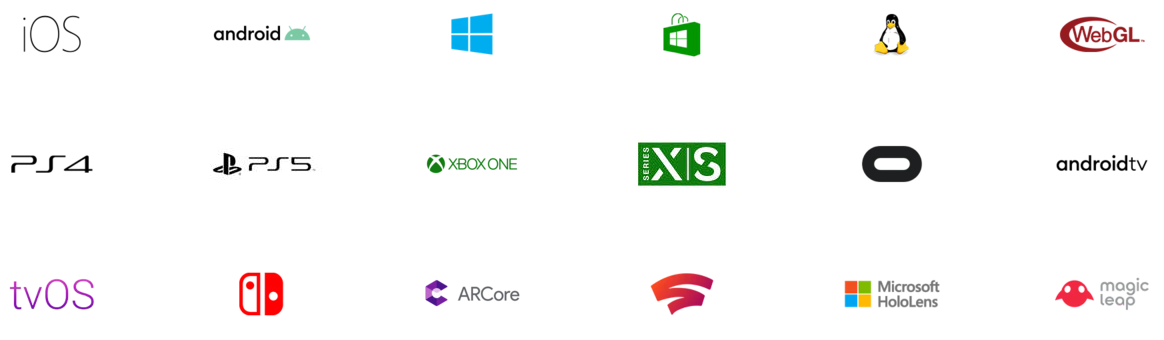
\includegraphics[width=1\textwidth]{Pictures/platforms.png}
	\caption{Platformy podporované Unity engine-om \cite{UnityMultiplatform}}
	\label{pic:UnityPlatforms}
\end{figure}

\subsection{Programovací jazyk C\# a architektúra .NET}
\label{sec:CsharpDotNet}
C\# \cite{CSharpLang} je objektovo orientovaný, typovo bezpečný programovací jazyk umožňujúci vytvárať aplikácie v .NET ekosystéme. Syntax jazyka C\# vychádza z programovacích jazykov C a C++. Narozdiel od nich ale ponúka vyššiu úroveň abstrakcie. Tá sa prejavuje napríklad na úrovni správy pamäte, čo z jazyka C\# robí voľbu číslo jedna pre začínajúcich programátorov, ktorí by si chceli skúsiť herný vývoj na vlastnej koži.

Architektúra .NET \cite{CSharpLang} potom ponúka okrem virtuálneho stroja CLR, ktorý vykonáva JIT kompiláciu IL kódu do strojových inštrukcií, aj sadu veľmi užitočných knižníc. Tieto knižnice sú organizované do menných priestorov a poskytujú širokú škálu metód vhodných napríklad na prácu so súbormi či sieťovou infraštruktúrou. Veľmi užitočné sú aj nástroje na syntaktickú analýzu XML prípadne platforma Windows Forms, ktorá sa v rámci mojej odbornej praxe vo firme Perun Creative ukázala byť vhodná hlavne na rýchlu tvorbu vývojárskych nástrojov. Kvôli limitáciám tejto technológie sa ale v budúcnosti plánuje prechod na systém WPF.
%pridaj aj winforms
\subsection{Verzovací systém Git}
\label{sec:Git}
Git \cite{ProGit} je open source distribuovaný systém na správu verzií vyvinutý Linusom Thorvaldsom a komunitou okolo OS Linux v roku 2005. Umožňuje vrátiť celý projekt alebo vybrané časti do predchádzajúceho stavu, porovnávať zmeny v súboroch, prípadne efektívnu kolaboráciu viacerých vývojárov na spoločnom projekte. Každý člen tímu má k dispozícií kompletný repozitár vrátane histórie jednotlivých súborov, čo pridáva ďalšiu vrstvu ochrany proti výpadkom a poruchám hardvéru. Po každom spustení príkazu \textit{commit} sa uloží aktuálny stav projektu, ktorý je možné spätne dohľadať v prípade nejakého problému.

S gitom je možné pracovať priamo z príkazového riadku ale pre väčšie projekty ako je aj hra Hobo: Tough Life je takýto prístup značne nepraktický a neefektívny. Existuje ale množstvo programov tretích strán, ktoré umožňujú pracovať s gitom z užívateľského rozhrania. Jedným takým je aj nástroj Sourcetree, s ktorým som v rámci mojej odbornej praxe pracoval.

Nakoľko git samotný nie je dobre prispôsobený na správu verzií veľkých súborov, bolo nutné využívať aj jeho rozšírenie Git LFS. 
\subsection{GitLab CI/CD}
\label{sec:GitLab}
Gitlab CI/CD je nástroj na vývoj softvéru prostredníctvom metodík ako:
\begin{itemize}
  \item \textbf{Continuous Integration (CI)} - 
  \item \textbf{Continuous Delivery (CD)} - 
  \item \textbf{Continuous Deployment (CD)} - 
\end{itemize}

\subsection{EOS}
\label{sec:Eos}
kkjnn
% End of section 3

% Section 4
\section{Popis projektov}
\label{sec:Projects}
U niektorych prebiehala tvorba inkrementalne a bola zavisla na spatnej vazbe bla bla.
% End of section 4

\printbibliography[title={Literatúra}, heading=bibintoc]
\end{document}
